%%%%%%%%%%%%%%%%%%%%%%%%%%%%%%%%%%%%%%%%%
% Class Notes Template
% LaTeX Template
% By: Ryan Grove
%%%%%%%%%%%%%%%%%%%%%%%%%%%%%%%%%%%%%%%%%

%----------------------------------------------------------------------------------------
%	PACKAGES AND OTHER DOCUMENT CONFIGURATIONS
%----------------------------------------------------------------------------------------

\documentclass[paper=a4, fontsize=11pt]{scrartcl} % A4 paper and 11pt font size

\usepackage[T1]{fontenc} % Use 8-bit encoding that has 256 glyphs
\usepackage{fourier} % Use the Adobe Utopia font for the document - comment this line to return to the LaTeX default
\usepackage[english]{babel} % English language/hyphenation
\usepackage{amsmath,amsfonts,amsthm} % Math packages

\usepackage{lipsum} % Used for inserting dummy 'Lorem ipsum' text into the template

\usepackage{sectsty} % Allows customizing section commands
\allsectionsfont{\centering \normalfont\scshape} % Make all sections centered, the default font and small caps

\usepackage{fancyhdr} % Custom headers and footers
\pagestyle{fancyplain} % Makes all pages in the document conform to the custom headers and footers
\fancyhead{} % No page header - if you want one, create it in the same way as the footers below
\fancyfoot[L]{} % Empty left footer
\fancyfoot[C]{} % Empty center footer
%\fancyfoot[R]{\thepage} % Page numbering for right footer
\renewcommand{\headrulewidth}{0pt} % Remove header underlines
\renewcommand{\footrulewidth}{0pt} % Remove footer underlines
\setlength{\headheight}{13.6pt} % Customize the height of the header

\numberwithin{equation}{section} % Number equations within sections (i.e. 1.1, 1.2, 2.1, 2.2 instead of 1, 2, 3, 4)
\numberwithin{figure}{section} % Number figures within sections (i.e. 1.1, 1.2, 2.1, 2.2 instead of 1, 2, 3, 4)
\numberwithin{table}{section} % Number tables within sections (i.e. 1.1, 1.2, 2.1, 2.2 instead of 1, 2, 3, 4)

\setlength\parindent{0pt} % Removes all indentation from paragraphs - comment this line for an assignment with lots of text

\usepackage{lastpage}
\usepackage{fancyhdr}
\cfoot{\thepage\ of \pageref{LastPage}}

\def\v{\hbox{$\mathbf v$}}
\def\w{\hbox{$\mathbf w$}}
\def\u{\hbox{$\mathbf u$}}
\def\x{\hbox{$\textbf{x}$}}
\def\z{\hbox{$\mathbf z$}}
\def\a{\hbox{$\mathbf a$}}
\def\b{\hbox{$\mathbf b$}}
\def\L{\hbox{$\mathcal L$}}
\def\C{\hbox{$\mathbb C$}}
\def\B{\hbox{$\mathcal B$}}
\def\R{\hbox{$\mathbb R$}}
\def\X{\hbox{$\underline X$}}
\def\Q{\hbox{$\mathbb Q$}}
\def\R{\hbox{$\mathbb R$}}
\def\N{\hbox{$\mathbb N$}}
\def\C{\hbox{$\mathbb C$}}
\def\0{\hbox{$\mathbf 0$}}
\def\Y{\hbox{$\underline Y$}}
\def\a{\hbox{$\mathbf a$}}
\def\u{\hbox{$\mathbf u$}}
\def\w{\hbox{$\mathbf w$}}
\def\y{\hbox{$\mathbf y$}}
\def\X{\hbox{$\underline X$}}
\def\dd{\hbox{$\partial $}}
\def\B{\hbox{$\mathcal B$}}
\def\F{\hbox{$\mathcal F$}}
\def\L{\hbox{$\mathcal L$}}
\def\M{\hbox{$\mathcal M$}}
\def\D{\hbox{$\mathscr {D}$}}
\def\RR{\hbox{$\mathscr{R}$}}
\def\I{\hbox{$\mathcal I$}}

\usepackage{amssymb}
%\theoremstyle{plain}
\usepackage[margin = .75in]{geometry}
\newtheorem{claim}{Claim}
\newtheorem{theorem}{Theorem}[section]
\newtheorem{lemma}[theorem]{Lemma}
\newtheorem{proposition}[theorem]{Proposition}
\newtheorem{corollary}[theorem]{Corollary}
\newtheorem{problem}[theorem]{Problem}
%\theoremstyle{definition}
\newtheorem{definition}[theorem]{Definition}
%\theoremstyle{remark}
\newtheorem{remark}[theorem]{Remark}
\newtheorem{remarks}[theorem]{Remarks}
\newtheorem{example}[theorem]{Example}
\newcommand{\ds}{\displaystyle}
\newcommand{\ZZ}{\mathbb{Z}}
\newcommand{\QQ}{\mathbb{Q}}
\newcommand{\e}{\varepsilon}
\newcommand{\bbf}{\textbf}
\newcommand{\p}{\parallel}
\usepackage{color}
\newcommand{\field}[1]{\mathbb{#1}}
\usepackage{amsmath}
\usepackage{amsthm}
\usepackage{amssymb}
\usepackage{mathrsfs}
\usepackage{cancel}
\usepackage{upgreek}
\usepackage{graphicx}
\usepackage{multirow}
\usepackage{setspace}
\usepackage{url}
\usepackage{subfigure}
\usepackage{enumerate}
\usepackage{cases}
\usepackage{mathrsfs}
\usepackage{rotating}

%----------------------------------------------------------------------------------------
%	TITLE SECTION
%----------------------------------------------------------------------------------------

\newcommand{\horrule}[1]{\rule{\linewidth}{#1}} % Create horizontal rule command with 1 argument of height

\title{	
\normalfont \normalsize 
\textsc{Ryan Grove, Clemson University, MATH1080 - 9} \\ [25pt] % Your name, university, class
\horrule{0.5pt} \\[0.4cm] % Thin top horizontal rule
\huge Section 11.10: Taylor and Maclaurin Series\\ % The assignment title
\horrule{2pt} \\[0.5cm] % Thick bottom horizontal rule
}

\author{Date:} % The due date

\date{\normalsize March 30, 2016} % A custom date

\begin{document}

\maketitle % Print the title

\begin{flushleft}
\begin{tabular}{l l}
Name: \rule{3.2in}{.01cm}  & {}%Table number: \rule{1in}{.01cm}\\
\end{tabular}
\end{flushleft}

%----------------------------------------------------------------------------------------
%	Lecture
%----------------------------------------------------------------------------------------

\section*{\textbf{Lecture:}}
In the preceding section we were able to find power series representations for a certain restricted class of functions. Here we investigate more general problems: Which functions have power series representations? How can we find such representations?\\
\indent

We start by supposing that $f$ is any function that can be represented by a power series
\[f(x) = c_0 + c_1(x-a) + c_2(x-a)^2 + c_3(x-a)^3 + c_4(x-a)^4 + \cdots, \quad |x-a| < R\]
\indent

\underline{Goal}: Determine what the coefficients $c_n$ must be in terms of $f$ (and its derivatives). To begin,

\[x=a \quad \implies \quad f(a) = c_0\]

Next, we differentiate the series term by term:

\[f'(x) = c_1 + 2c_2(x-a) + 3c_3(x-a)^2 + 4c_4(x-a)^3 + \cdots, \quad |x-a|<R \]

and now
\[x=a \quad \implies \quad f'(a) = c_1\]

Differentiating the series again we have:

\[f''(x) = 2c_2 + 2\cdot 3 c_3 (x-a) + 3\cdot 4 c_4 (x-a)^2 + \cdots, \quad |x-a|<R\]

and now
\[x=a \quad \implies \quad f''(a) = 2c_2\]

Applying the same procedure one more time gives:

\[f'''(x) = 2\cdot 3 c_3 + 2\cot 3 \cdot 4 c_4 (x-a) + 3\cdot 4 \cdot 5 c_5 (x-a)^2 + \cdots, \quad |x-a|<R\]

and now
\[f'''(a) = 2\cdot 3 c_3 = 3! c_3\]

By now you can see the pattern. If we continue to differentiate and substitute $x=a$, we obtain

\begin{align*}
f^{(n)}(a) &= 2\cdot 3 \cdot 4 \cdot \cdots \cdot n c_n = n! c_n\\
\text{ }\\
\implies \quad \quad c_n &= \ds\frac{\hspace{0.75in}}{\hspace{0.5in}}\\
\end{align*}
\indent

This formula remains valid even for $n=0$ if we adopt the conventions that $0!=1$ and $f^{(0)} = f$. Thus we have proved the following theorem.\\

\fbox{
  \parbox{\textwidth}{
  \vspace{5pt} \textbf{Theorem 1:} If $f$ has a power series representation (expansion) at $a$, that is, if
  
  \[f(x) = \ds\sum_{n=0}^\infty c_n (x-a)^n, \quad |x-a|<R\]
  
  then its coefficients are given by the formula:
  
  \[c_n = \ds\frac{f^{(n)}(a)}{n!}.\]
  
  }}
  \indent\\
  \indent
  
  Substituting this formula for $c_n$ back into the series, we see that \textit{if} $f$ has a power series expansion at $a$, then it must be of the following form:\\
  \indent
  
 \fbox{
  \parbox{\textwidth}{
  \vspace{5pt} 
  \begin{align*}
  f(x) &= \ds\sum_{n=0}^\infty \ds\frac{f^{(n)}(a)}{n!}(x-a)^n\\
  &= f(a) + \ds\frac{f'(a)}{1!}(x-a) + \ds\frac{f''(a)}{2!}(x-a)^2 + \ds\frac{f'''(a)}{3!}(x-a)^3+\cdots
  \end{align*}
  
  }}
  \indent\\
  \indent
  
  This series is called the \textbf{Taylor series of the function} $\mathbf{f}$ \textbf{at} $\mathbf{a}$ (or \textbf{centered at} $\mathbf{a}$ or \textbf{about} $\mathbf{a}$). For the special case \underline{\hspace{0.75in}} the Taylor series becomes\\
  \indent
  
\fbox{
  \parbox{\textwidth}{
  \vspace{5pt}
  
  \[f(x) = \ds\sum_{n=0}^\infty \ds\frac{f^{(n)}(0)}{n!}x^{n} = f(0) + \ds\frac{f'(0)}{1!} + \ds\frac{f''(0)}{2!}x^2 + \cdots\]
  }}
  \indent\\
  \indent
  
  This case arises frequently enough that it is given the special name \underline{\hspace{1in}} \underline{\hspace{1in}}. \\
  \indent
  
  That is, a \textbf{Maclaurin Series} is a \textbf{Taylor Series} centered at $a=0$.\\
  \indent
  
  \newpage
  
  \underline{Example 1}: Find the Maclaurin series of the function $f(x)=e^x$ and its radius of convergence.\\
  \indent
  
  \vspace{4in}
  
  \newpage
  
  \textbf{NOTE:} We have shown that \textit{if} $f$ can be represented as a power series about $a$, then $f$ is equal to the sum of its Taylor series. But there exist functions that are not equal to the sum of their Taylor series. So the question is: Under what circumstances is a function equal to the sum of its Taylor series? That is, when is
  
  \[f(x) = \ds\sum_{n=0}^\infty \ds\frac{f^{(n)}(a)}{n!}(x-a)^n ?\]
  
  As with any convergent series, this means that $f(x)$ is the limit of the sequence of partial sums. In the case of the Taylor series, the partial sums are:
  
  \begin{align*}
  T_n(x) &= \ds\sum_{i=0}^n \ds\frac{f^{(i)}(a)}{i!}(x-a)^i\\
  &= f(a) + \ds\frac{f'(a)}{1!}(x-a) + \ds\frac{f''(a)}{2!}(x-a)^2 + \cdots + \ds\frac{f^{(n)}(a)}{n!}(x-a)^n
  \end{align*}
  \indent
  
  Notice that $T_n$ is a polynomial of degree $n$ called the \underline{\hspace{3in}}. For instance, for the exponential function $f(x)=e^x$, the result of Example 1 shows that the Taylor polynomials at 0 (or Maclaurin polynomials here) with $n=1,2, \text{ and } 3$ are
  
  \[T_1(x) = 1+x, \quad \quad T_2(x) = 1+x+\ds\frac{x^2}{2!}, \quad \quad T_3(x) = 1  + x + \ds\frac{x^2}{2!} + \ds\frac{x^3}{3!}\]
  \indent
  
  The graphs of the exponential function and these three Taylor polynomials are drawn in Figure 1.
  
  \[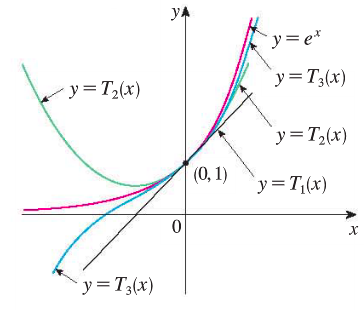
\includegraphics[scale=0.5]{11-10pic1.png} \quad \quad 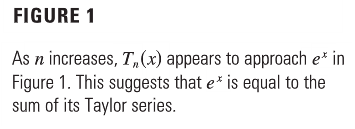
\includegraphics[scale=0.5]{11-10pic2.png}\]
  
 In general, $f(x)$ is the sum of its Taylor series if
 
 \[f(x) = \ds\lim_{n\to\infty}T_n(x).\]
 
We define $R_n(x) = f(x) - T_n(x)$ to be the \underline{\hspace{1.2in}} of the Taylor series. If we can show somehow that $\ds\lim_{n\to\infty}R_n(x) = 0$, then it follows that

\[\ds\lim_{n\to\infty}T_n(x) = \hspace{3.5in}\]

We have therefore proved the following theorem.
  
\fbox{
  \parbox{\textwidth}{
  \vspace{5pt} \textbf{Theorem 2}: If $f(x)=T_n(x) + R_n(x)$, where $T_n$ is the $n^{\text{th}}$-degree Taylor polynomial of $f$ at $a$ and 
  \[\ds\lim_{n\to\infty}R_n(x)=0\]
  
  for $|x-a|<R$, then $f$ is equal to the sum of its Taylor series on the interval $|x-a|<R$.\\
  
  }}
  \indent\\
  \indent
  
  In trying to show that $\ds\lim_{n\to\infty}R_n(x)=0$ for a specific function $f$, we usually use the following Theorem.\\
  \indent
  
  \fbox{
  \parbox{\textwidth}{
  \vspace{5pt} \textbf{Theorem 3 (Taylor's Inequality):} If $|f^{(n+1)}(x)|\leq M$ for $|x-a|\leq d$, then the remainder $R_n(x)$ of the Taylor series satisfies the inequality
  
  \[|R_n(x)|\leq \ds\frac{M}{(n+1)}|x-a|^{n+1} \quad \text{ for } |x-a|\leq d\]
  
  }}
  \indent\\
  \indent
  
%  \textbf{NOTE:} In Section 11.11 we will explore the use of Taylor's Inequality in approximating functions. Our immediate use of it is in conjunction with Theorem 2.\\
%  \indent
%  
%  In applying Theorems 2 and 3 it is often helpful to make use of the following fact:
%  
%  \[\boxed{\quad \ds\lim_{n\to\infty}\ds\frac{x^n}{n!} = 0 \quad \text{ for every real number } x \quad}\]
%  
%  That is, factorial overpowers exponential. This is true because we know from Example 1 that the series $\ds\sum \ds\frac{x^n}{n!} $ converges for all $x$ and so its $n$th term approaches 0.\\
%  \indent
%  
%  \newpage
%  
%  \underline{Example 2}: Prove that $e^x$ is equal to the sum of its Maclaurin series.\\
%  \indent
%  
%  
%  
%  \vspace{6in}
  
%  In particular, for $x=1$ we obtain the following expression for the number $e$ as a sum of an infinite series:
%  
%  \[\boxed{ \quad e= \ds\sum_{n=0}^\infty \ds\frac{1}{n!} = 1 + \ds\frac{1}{1!} + \ds\frac{1}{2!} + \ds\frac{1}{3!} + \cdots \quad }\]
%  \indent
  
  
  \underline{Example 4}: Find the Maclaurin series for $\sin x$.\\
  \indent
  
  \vspace{6in}
  
\fbox{
  \parbox{\textwidth}{
  \vspace{5pt}
  \begin{align*}
  \sin x &= x - \ds\frac{x^3}{3!} + \ds\frac{x^5}{5!} - \ds\frac{x^7}{7!} + \cdots \\
  &= \ds\sum_{n=0}^\infty (-1)^n \ds\frac{x^{2n+1}}{(2n+1)!} \quad \text{for all $x$}
  \end{align*}
  }}
  
  
  \newpage
  
  \underline{Example 5}: Find the Maclaurin series for $\cos x$.\\
  \indent
  
  \vspace{7in} 
  
  \fbox{
  \parbox{\textwidth}{
  \vspace{5pt}
  \begin{align*}
  \cos x &= 1 - \ds\frac{x^2}{2!} + \ds\frac{x^4}{4!} - \ds\frac{x^6}{6!} + \cdots \\
  &= \ds\sum_{n=0}^\infty (-1)^n \ds\frac{x^{2n}}{(2n)!} \quad \text{for all $x$}
  \end{align*}
  }}
  \indent\\
  \indent
  
  \newpage
  
  \underline{Example 6}: Find the Maclaurin series for the function $f(x) = x\cos x$.\\
  \indent
  
  \vspace{2in}
  
  \underline{Example 7}: Represent $f(x) = \sin x$ as the sum of its Taylor series centered at $\ds\frac{\pi}{3}$.\\
  \indent
  
  \newpage
  
  \underline{Example 8}: Find the Maclaurin series for $f(x) = (1+x)^k$, where $k$ is any real number.\\
  \indent
  
  
  \vspace{7in}
  
  This series is called the \underline{\hspace{1in}} \underline{\hspace{1in}}. \\
  \indent
  
\fbox{
  \parbox{\textwidth}{
  \vspace{5pt}
  \textbf{The Binomial Series:} If $k$ is any real number and $|x|<1$, then
  
  \[(1+x)^k = \ds\sum_{n=0}^\infty \binom{k}{n} x^n = 1 + kx + \ds\frac{k(k-1)}{2!}x^2 + \ds\frac{k(k-1)(k-2)}{3!}x^3 + \cdots\]
  }}
  \indent\\
  \indent
  
  \newpage 
  We collect in the following table, for future reference, some important Maclaurin series that we have derived in this section and the preceding one.\\
  \indent
  
  \[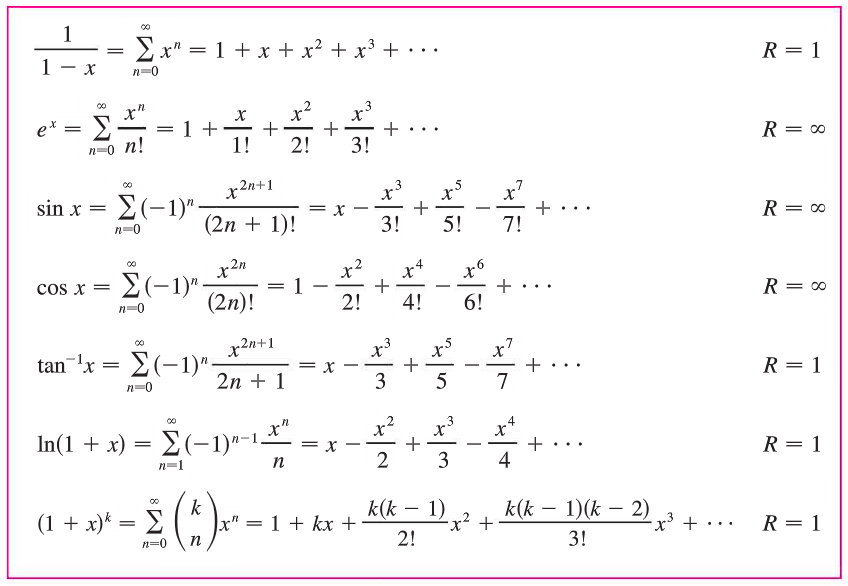
\includegraphics[scale=0.5]{11-10pic3.png}\]
  \indent
  
  \underline{Example 10}: Find the sum of the series $\ds\frac{1}{1\cdot 2} - \ds\frac{1}{2\cdot 2^2} + \ds\frac{1}{3\cdot 2^3} - \ds\frac{1}{4\cdot 2^4} + \cdots$.\\
  \indent
  
  \textbf{SOLUTION}: Writing the given series in sigma notation we have:\\
  \indent
  
  \[ \text{ }\]
  \indent\\
  \indent
  
  Then from the table above we see that this series matches the entry for $\ln(1+x)$ with \underline{\hspace{0.75in}}. So,
  
  \[\ds\sum_{n=1}^\infty (-1)^{n-1}\ds\frac{1}{n\cdot 2^n} = \underline{\hspace{1.5in}} = \underline{\hspace{1in}}.\]
  
  \newpage
  
  The function $f(x)=e^{-x^2}$ can't be integrated by techniques discussed so far because its antiderivative is not an elementary function. But we can integrate it by first expressing it as a power series and then integrating term by term as in the following example.\\
  \indent
  
  \underline{Example 11}:
  \begin{enumerate}
  \item[(a)] Evaluate $\ds\int e^{-x^2}dx$ as an infinite series.\\
  \item[(b)] Evaluate $\ds\int_{0}^1 e^{-x^2}dx$ correct to within an error of 0.001.
  \end{enumerate}
  \indent
  
  
  
  \newpage
  
  \underline{Example 12}: Evaluate $\ds\lim_{x\to 0}\ds\frac{e^x - 1 - x}{x^2}$ without using L'Hospital's Rule.\\
  \indent
  
  
  


%----------------------------------------------------------------------------------------

\end{document}